%%%%%%%%%%%%%%%%%%%%%%%%%%%%%%%%%%%%%%%%%
% Programming/Coding Assignment
% LaTeX Template
%
% This template has been downloaded from:
% http://www.latextemplates.com
%
% Original author:
% Ted Pavlic (http://www.tedpavlic.com)
%
% Note:
% The \lipsum[#] commands throughout this template generate dummy text
% to fill the template out. These commands should all be removed when 
% writing assignment content.
%
% This template uses a Perl script as an example snippet of code, most other
% languages are also usable. Configure them in the "CODE INCLUSION 
% CONFIGURATION" section.
%
%%%%%%%%%%%%%%%%%%%%%%%%%%%%%%%%%%%%%%%%%

%----------------------------------------------------------------------------------------
%	PACKAGES AND OTHER DOCUMENT CONFIGURATIONS
%----------------------------------------------------------------------------------------

\documentclass{article}

\usepackage{fancyhdr} % Required for custom headers
\usepackage{lastpage} % Required to determine the last page for the footer
\usepackage{extramarks} % Required for headers and footers
\usepackage[usenames,dvipsnames]{color} % Required for custom colors
\usepackage{graphicx} % Required to insert images
\usepackage{listings} % Required for insertion of code
\usepackage{courier} % Required for the courier font
\usepackage{pgfgantt}

% Margins
\topmargin=-0.45in
\evensidemargin=0in
\oddsidemargin=0in
\textwidth=6.5in
\textheight=9.0in
\headsep=0.3in

\linespread{1.1} % Line spacing

% Set up the header and footer
\pagestyle{fancy}
\lhead{\hmwkAuthorName} % Top left header
\chead{\hmwkTitle} % Top center head
\rhead{\hmwkClass } % Top right header
\lfoot{} % Bottom left footer
\cfoot{} % Bottom center footer
\rfoot{Page\ \thepage\ of\ \protect\pageref{LastPage}} % Bottom right footer
\renewcommand\headrulewidth{0.4pt} % Size of the header rule
\renewcommand\footrulewidth{0.4pt} % Size of the footer rule

\setlength\parindent{0pt} % Removes all indentation from paragraphs

%----------------------------------------------------------------------------------------
%	CODE INCLUSION CONFIGURATION
%----------------------------------------------------------------------------------------

\definecolor{MyDarkGreen}{rgb}{0.0,0.4,0.0} % This is the color used for comments
\lstloadlanguages{Java} % Load Java syntax for listings, for a list of other languages supported see: ftp://ftp.tex.ac.uk/tex-archive/macros/latex/contrib/listings/listings.pdf
\lstset{language=Java, % Use Java in this example
        frame=none, % Single frame around code
        basicstyle=\small\ttfamily, % Use small true type font
        keywordstyle=[1]\color{Blue}\bf, % Perl functions bold and blue
        keywordstyle=[2]\color{Purple}, % Perl function arguments purple
        keywordstyle=[3]\color{Blue}\underbar, % Custom functions underlined and blue
        identifierstyle=, % Nothing special about identifiers                                         
        commentstyle=\usefont{T1}{pcr}{m}{sl}\color{MyDarkGreen}\small, % Comments small dark green courier font
        stringstyle=\color{Purple}, % Strings are purple
        showstringspaces=false, % Don't put marks in string spaces
        tabsize=8, % 5 spaces per tab
        %
        % Put standard Perl functions not included in the default language here
        morekeywords={rand},
        %
        % Put Perl function parameters here
        morekeywords=[2]{on, off, interp},
        %
        % Put user defined functions here
        morekeywords=[3]{test},
       	%
        morecomment=[l][\color{Blue}]{...}, % Line continuation (...) like blue comment
        numbers=left, % Line numbers on left
        firstnumber=1, % Line numbers start with line 1
        numberstyle=\tiny\color{Blue}, % Line numbers are blue and small
        stepnumber=100 % Line numbers go in steps of 5
}


%----------------------------------------------------------------------------------------
%	DOCUMENT STRUCTURE COMMANDS
%	Skip this unless you know what you're doing
%----------------------------------------------------------------------------------------

% Header and footer for when a page split occurs within a problem environment
\newcommand{\enterProblemHeader}[1]{
\nobreak\extramarks{#1}{#1}\nobreak
\nobreak\extramarks{#1}{#1}\nobreak
}

% Header and footer for when a page split occurs between problem environments
\newcommand{\exitProblemHeader}[1]{
\nobreak\extramarks{#1}{#1 continued on next page\ldots}\nobreak
\nobreak\extramarks{#1}{}\nobreak
}

\setcounter{secnumdepth}{0} % Removes default section numbers
\newcounter{homeworkProblemCounter} % Creates a counter to keep track of the number of problems

\newcommand{\homeworkProblemName}{}
\newenvironment{homeworkProblem}[1][
 \arabic{homeworkProblemCounter}]{ % Makes a new environment called homeworkProblem which takes 1 argument (custom name) but the default is "Problem #"
\stepcounter{homeworkProblemCounter} % Increase counter for number of problems
\renewcommand{\homeworkProblemName}{#1} % Assign \homeworkProblemName the name of the problem
\section{\homeworkProblemName} % Make a section in the document with the custom problem count
\enterProblemHeader{} % Header and footer within the environment
}{
\exitProblemHeader{} % Header and footer after the environment
}

\newcommand{\problemAnswer}[1]{ % Defines the problem answer command with the content as the only argument
\noindent\framebox[\columnwidth][c]{\begin{minipage}{0.98\columnwidth}#1\end{minipage}} % Makes the box around the problem answer and puts the content inside
}

\newcommand{\homeworkSectionName}{}
\newenvironment{homeworkSection}[1]{ % New environment for sections within homework problems, takes 1 argument - the name of the section
\renewcommand{\homeworkSectionName}{#1} % Assign \homeworkSectionName to the name of the section from the environment argument
\subsection{\homeworkSectionName} % Make a subsection with the custom name of the subsection
\enterProblemHeader{\homeworkProblemName\ [\homeworkSectionName]} % Header and footer within the environment
}{
\enterProblemHeader{\homeworkProblemName} % Header and footer after the environment
}


%----------------------------------------------------------------------------------------
%	NAME AND CLASS SECTION
%----------------------------------------------------------------------------------------

\newcommand{\hmwkTitle}{Final Report} % Assignment title
\newcommand{\hmwkDueDate}{29th April 2016} % Due date
\newcommand{\hmwkClass}{COMP30050} % Course/class
\newcommand{\hmwkClassTime}{Software Engineering Project 3} % Class/lecture time
\newcommand{\hmwkClassInstructor}{Dr. Tony Veale} % Teacher/lecturer
\newcommand{\hmwkAuthorName}{Lamp} % Your name

%----------------------------------------------------------------------------------------
%	TITLE PAGE
%----------------------------------------------------------------------------------------

\title{
\vspace{2in}
\textmd{\textbf{\hmwkClass:\ \hmwkClassTime}}\\
\normalsize\
\vspace{0.1in}\large{\textit{\hmwkClassInstructor}}\\
\vspace{0.2in}
\textmd{\textbf{\hmwkTitle}}\\
\small{Due\ on\ \hmwkDueDate}\\
\vspace{.5in}
}

\author{\textbf{\hmwkAuthorName}\\
Joe Duffin - 13738019\\
Edwin Keville - 13718661\\
Niamh Kavanagh - 12495522\\
Gerard Fogarty - 13303911 (\textit{the lost lamp})
}

\date{} % Insert date here if you want it to appear below your name

%----------------------------------------------------------------------------------------

\begin{document}
\begin{titlepage}
\maketitle
\thispagestyle{empty}
\end{titlepage}

\newpage
%----------------------------------------------------------------------------------------
%	TABLE OF CONTENTS
%----------------------------------------------------------------------------------------

%\setcounter{tocdepth}{1} % Uncomment this line if you don't want subsections listed in the ToC

\newpage
\tableofcontents
\newpage

%----------------------------------------------------------------------------------------

\begin{homeworkProblem}[Introduction (Spec of project)]
As part of our third year software engineering module, all students were required to develop a stochastic search project allocation system. This is to be completed in groups,  with the initial framework designed by each individual member through weekly assignments, before amalgamating each member's solution and adding the functionality of two different solution algorithms. The end result produces an optimal allocation of data in a user-friendly format which can be saved as desired.

The project itself involves reading in a list of students and their ranked list of preferences for final year projects within computer science. Some students may have a project preassigned to them, in which case they will have no other preferences and will not be altered in the allocation process. Any students without a preassigned project will then be assigned a project using our chosen algorithms in an attempt to minimize overall student disappointment. 

The proposed solution for this mapping of students to projects was developed using both a simulated annealing and a genetic algorithm. The simulated annealing approach provides a singular solution, which it adapts through a serious of changes to individual student-project mappings until a good viable solution is achieved. The genetic algorithm creates a population of random solutions, with solutions merging and being culled until a single optimal solution is reached. 

To allow our software to be user-friendly, we created a Graphical User Interface and a Command Line Interface. The GUI allows users to load the data file of their choice and run our hybrid algorithm composed of a genetic algorithm populated by simulated annealing solutions, then gives the option to save these results into a spreadsheet format with the energy of the solution displayed at the bottom. The CLI uses command line arguments provided by the user to specify the desired input file, which algorithm to be used, the parameters for each algorithm and the desired format of the output file.

The following report details our software in full, discussing both algorithms used and the hybrid we created of both, a user manual for accessibility, and the entire development process undertook to create the final project.









\end{homeworkProblem}
\newpage

%----------------------------------------------------------------------------------------

\begin{homeworkProblem}[What we produced/interfaces]

One Gui and 3 command line interfaces. 
We wanted a fine mix of an ultimate solution, but also lots of modularity and re-usability.

\begin{homeworkSection}{The Graphical User Interface}
The hybrid solution, the actual submission.
\end{homeworkSection}

\begin{homeworkSection}{The Command Line Version}
hi
\end{homeworkSection}








\end{homeworkProblem}
\newpage

%---------------------------------------------------------------------------------------
\begin{homeworkProblem}[Class Diagrams]

\begin{homeworkSection}{The Gui with Simulated Annealing and the Genetic Algorithm}
The Gui relies on the Link to get access to both the Simulated Annealing and Genetic Algorithms.  The 1 to 1 relationships between the CallBackListener and the algorithms allow the algorithms to update the status bar and text on the Gui.
\begin{center}
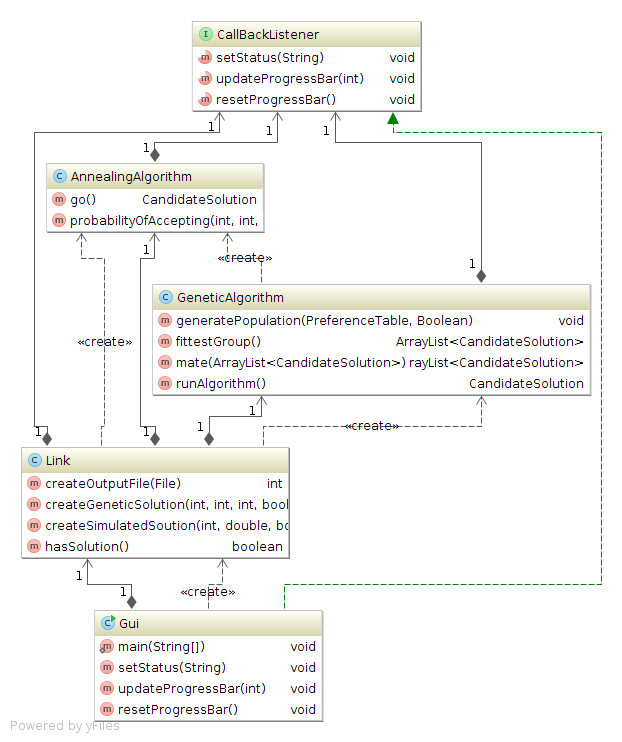
\includegraphics[width=0.76\columnwidth]{Gui} % Example image
\end{center}
\end{homeworkSection}
\newpage
\begin{homeworkSection}{Cli for Simulated Annealing}
The Cli has a 1 to 1 relationship with the Link, which here is shown to give access to the Simulated Annealing algorithm. This, in turn, has a 1 to 1 relation ship with a Candidate Solution which it permutes. 
\begin{center}
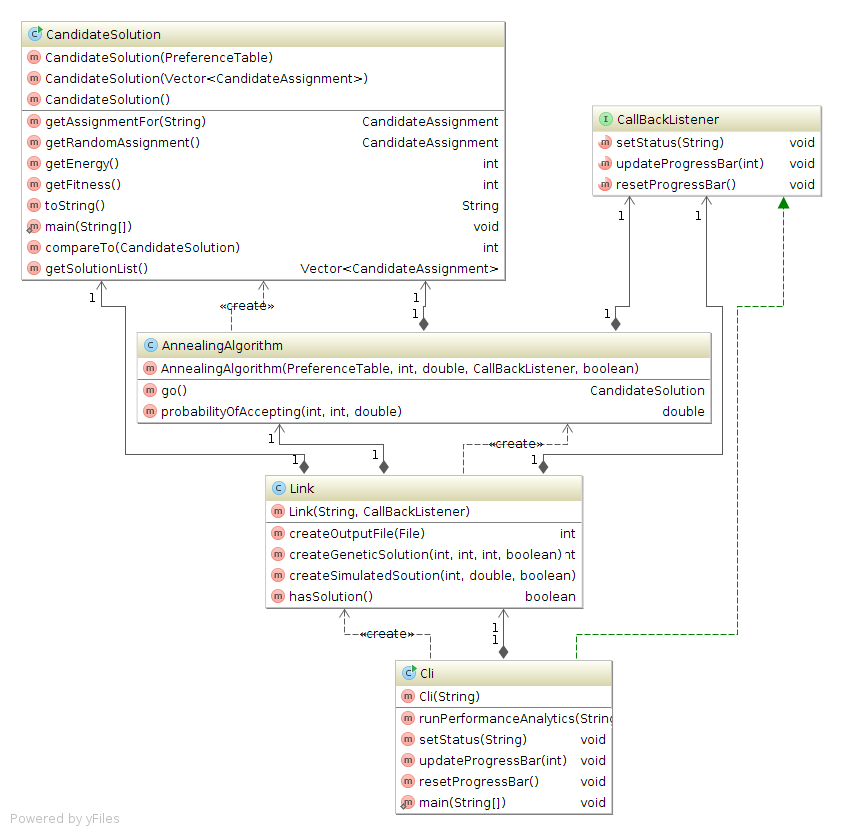
\includegraphics[width=0.99\columnwidth]{Cli-Annealing} % Example image
\end{center}
\end{homeworkSection}
\newpage
\begin{homeworkSection}{Cli for the Genetic Algorithm}
When the user elects to use the Genetic Algorithm the 1 to 1 relationship between the Link and the Genetic Algorithm is used. In the diagrams below the inheritance relationship the ChildCandidateSolution and the CandidateSolution is evident.
\begin{center}
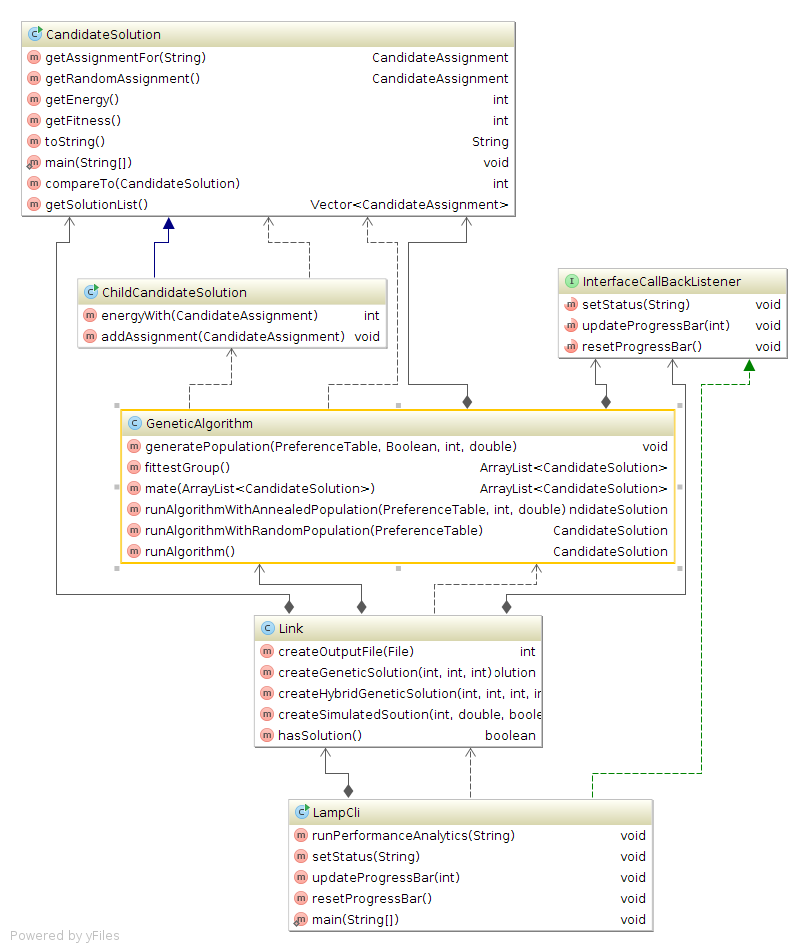
\includegraphics[width=0.99\columnwidth]{Cli-Genetic} % Example image
\end{center}
\end{homeworkSection}

\newpage
%------------------------------------------------------------------------------------------
\begin{homeworkProblem}[Performance Analysis]
Each algorithm has its own set of parameters which are needed and these have a significant effect on the overall energy of the given solution. We wanted our Gui to be a simple no frills program to give the ultimate solution so we removed the option of user input parameters. They are set as constant. In order to determine the best constants we ran overnight tests, subjecting each algorithm to a barrage of parameters. These results can be reproduced using the '-analyse' tag with in Cli version of our code. 
\\\\
If an advanced user wishes to specify their own parameters, the Cli version of our program will facilitate that.

\begin{homeworkSection}{The Genetic Alogrithm}
The Genetic Algorithm has 3 parameters:
\begin{itemize}
\item The initial population size
\item How may of the population to choose for mating (The top N)
\item The number of generations the population should evolve through
\end{itemize}
The overnight test yielded the following graph.

\begin{center}
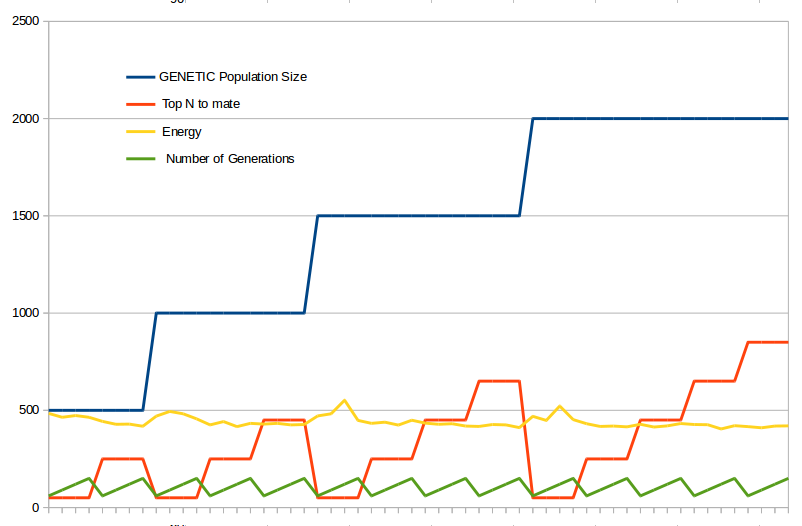
\includegraphics[width=0.9\columnwidth]{GaPerf} % Example image
\end{center}

The algorithm was ran with a variety of population sizes, number to mate and number of generation and the best parameters which gave the lowest energy were extracted.
\begin{description}
\item[Population Size:] 2000
\item[Top N:] 650
\item[Number of Generations:] 120
\end{description}

\end{homeworkSection}


\begin{homeworkSection}{The Simulated Annealing alogrithms}
The Simulated Annealing Algorithm has 2 parameters:
\begin{itemize}
\item The initial temperature of the solution
\item The amount the solution cools on each iteration.
\end{itemize}
The overnight test yielded the following graph.
\begin{center}
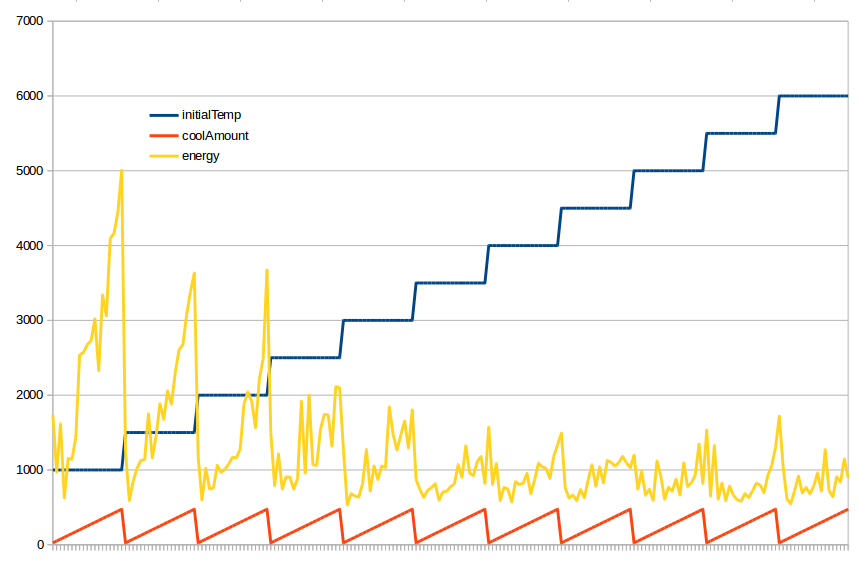
\includegraphics[width=0.9\columnwidth]{SaPerf} \\
\end{center}

The algorithm was ran with a variety of cooling amounts for a variety of initial temperatures. The cool amount has been scaled by a factor of 100 for clarity. The best parameters are shown below.
\begin{description}
\item[Initial Temperature] 3000
\item[Cooling Amount] 0.5
\end{description}

\end{homeworkSection}



\end{homeworkProblem}
\newpage
%------------------------------------------------------------------------------------------
\begin{homeworkProblem}[Development Phases/Issues]



\begin{homeworkSection}{The Genetic Algorithm}

mate was the biggun\\
initially when mating 2 solutions we choose the 'happiest' corresponding assignments from each and created a new assignment with these. Each assignment was independently better, the solution as a whole was pants as there were lots of penalties incurred.\\
We move to considering a complete child solution and used the notion of 'happier with' to determine which parent's assignment should be used.\\
\\
extras\\
checking for duplicates manually (winning) - bad\\
mutations, several attempts - bad\\
\end{homeworkSection}

\begin{homeworkSection}{The Simulated Annealing Algorithm}
The key turning point being understanding the relationship between initial tmeperature and cooling amount. Number iterations is a function of these two.
\end{homeworkSection}

\begin{homeworkSection}{The Gui} 
The Gui was initially overcomplicated,,, after performance analysis we determined none of this was necessary. We elected for a simple LOAD GO SAVE option, with an epic title bar. It allows the user to create the ultimate solution, (or very close too) insert percentage.

\begin{center}
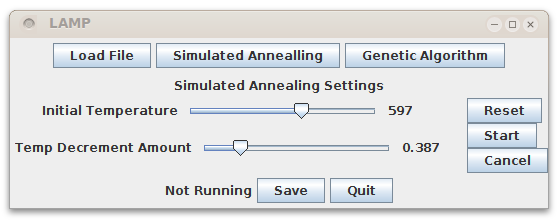
\includegraphics[width=0.86\columnwidth]{ComplexGui} % Example image
\end{center}

\end{homeworkSection}{}







\end{homeworkProblem}
\newpage

%---------------------------------------------------------------------------------------
\begin{homeworkProblem}[Our Development Model]



\begin{homeworkSection}{Not sure what needs to go in here}

\end{homeworkSection}






\end{homeworkProblem}
\newpage

%---------------------------------------------------------------------------------------
\begin{homeworkProblem}[Technical Details Of Note]


\begin{homeworkSection}{Our Design Pattern}
In keeping with our core values of simplicity and re-usability we tried to use a very modular design pattern. We identified two distinct types of classes that we created, worker classes and interfaces (the algorithms and the Cli/Gui respectively). An interface invokes methods on a worker. In order to modularise this we created a Link class. This is a pivotal class in our design. Every method call from an interface must go through the link. This gives the ability to pair any interface with any algorithm with ease. Once an interface has access to a Link it can call upon either or both of the algorithms as is necessary. The linear flow of our design pattern is very evident below.
\begin{center}
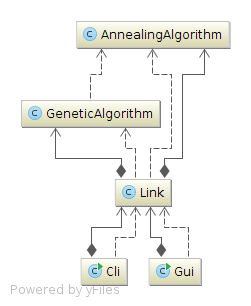
\includegraphics[width=0.27\columnwidth]{DesignPattern} % Example image
\end{center}
\end{homeworkSection}


\begin{homeworkSection}{Callback listeners}
Independent communication between classes is typically one directional. Usually a class invokes a method on one of the classes that it has references to and a single value is returned upon completion. Sometimes the need for interaction with the calling class is needed during execution of the called method; this is where callback listeners come in. They provide the ability for a method to invoke a method on the calling class.\\\\
Use of callback listeners:
\begin{enumerate}
\item The listener is ultimately an interface. It declares which methods in the calling class are available to class containing the called method.
\item The calling class implements each of the methods declared in this interface.
\item When creating an instance of a class, whose methods will be called at some point, a reference to the calling class is passed using the "this" keyword to the classes constructor.
\item That class, which needs the reverse communication path, then instantiates an object of type callback listener with the passed reference. 
\item This allows method calls back to the calling class during execution and also keeps encapsulation tight as it does not provide the full public interface of the calling class.
\item Callback listeners can also be used with threads to alert the class which created the thread of completion or another significant event.
\end{enumerate}
In our project methods in the algorithm classes are invoked by either of the interface classes (via the Link). We used a callback listener to allow both the Genetic and Simulated Annealing algorithms to invoke methods on which ever interface invoked the algorithm. The callback listener is a direct connection straight back to the calling class. 
\\We used the listener to update the progress bar every time 10 percent of the total number of iterations have been completed and also when the status bar needed updating with new information. Our two interfaces, the Cli and Gui, both implement the callback listener and have their own respective versions of the status bar and progress bar.

\end{homeworkSection}
\begin{homeworkSection}{Inheritance}
When building software, in order to efficiently utilise the classes at one's disposal. it is always important to be mindful of potential inheritance relationships. An inheritance relationship gives a subclass access to the methods and fields of the superclass. Inheritance is used when needing to add case specific functionality to a class, i.e. extra functionality that would otherwise bloat other clients of the class. 
\\\\
We identified a need to subclass the CandidateSolution class when creating the Genetic Algorithm. The Genetic Algorithm has to build a CandidateSolution one project at a time and also query the potential fitness of that solution during the building phase. This led to the creation of the ChildCandidateSolution class, which inherits from CandidateSolution, with two extra methods, evident below.
\begin{center}
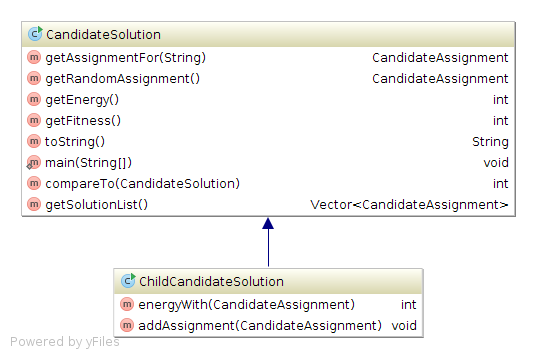
\includegraphics[width=0.60\columnwidth]{Inheritance} % Example image
\end{center}

\end{homeworkSection}

\begin{homeworkSection}{Threads} 
By default programs run on one main thread. They have one time line, one stream of execution, on which the programs instructions are carried out consecutively. Sometimes, when expensive routines are needed to be called it's advantageous to put them on their own thread, their stream of execution. When the routine is complete is typically not known, but it will complete at some point, (assuming no runtime/logic errors). Callback listeners can be used to signal the main thread of completion or some other significant event. 
\\\\
In our project, the Cli runs in only one thread, and procedurally runs the algorithm and prints the the console to indicate its progress. During execution the user has no interactivity with the program as it's main thread is blocked by the expensive task of computing a solution.\\
When we designed the Gui it became evident that a separate execution thread was needed as there are two tasks to complete. The Jframe that is the Gui needs redrawing with the progress bar updates and the algorithm has to be executed. We created a separate thread on which the algorithm would run, allowing these two tasks to done concurrently.
\end{homeworkSection}{}







\end{homeworkProblem}
\newpage

%---------------------------------------------------------------------------------------

\begin{homeworkProblem}[Team Development]

what we changed\\
what we liked/didnt,\\
stuckto/deviated from interim\\

\begin{homeworkSection}{What went well}
the night out and the burgers

\end{homeworkSection}

\begin{homeworkSection}{What didn't go so well}
everything else
\end{homeworkSection}


\begin{homeworkSection}{Who did what}
everything else
\end{homeworkSection}{}


\end{homeworkProblem}



\newpage









\end{homeworkProblem}
\newpage

%---------------------------------------------------------------------------------------

\begin{homeworkProblem}[The Team Night Out]
\begin{homeworkSection}{Burgers and Drama}
The development of a large software project involves both individual and group contributions. Many large tasks were broken up into smaller subsections which were divided between the team members. These were researched and brainstormed individually before meeting as a group and developing solutions together. 

To keep morale high while we worked through the assignment, we organized a team bonding night between the interim report and the submission of the final report. This took place after a long group coding session in college where the bones of both algorithms were written. We felt that an evening of discussion on topics other than the software project would help keep us connected as a group, which would improve overall work ethic and quality of code produced.

The team night out involved travelling together into town for a large dinner, before returning to UCD campus for a production of The Nightman Cometh (an episode of the popular TV show It's Always Sunny in Philadelphia) by UCD's DramaSoc. A night off from code development and report writing was well deserved and earned, and allowed for the team to work harder upon our return to college the next day.
\end{homeworkSection}
\end{homeworkProblem}

%----------------------------------------------------------------------------------------
\begin{homeworkProblem}[A Sad Day For Lamp]

\begin{homeworkSection}{The loss of a team member}
As a young adult, college can often be a very stressful and time consuming environment to be in. A large amount of students are dropping out of all courses, with 23\% of students entering the computer science program in UCD not progressing past their first year. Unfortunately for Team Lamp, we experienced a loss of a member partway through the development process.

Team Lamp started off well, producing strong weekly assignments by each team member. Sadly, we found that as time passed, one member was slowly fading off the radar and was no longer contributing towards the module in both individual assessments and team projects. Gerard Fogarty, our lost Lamp, has unfortunately not been a presence within the team for several weeks. 

Team Lamp has persevered through this loss, providing what we feel is still a marketable software solution to this module's brief. Although this module heavily suggested teams of four to produce a solid working solution, we feel that we overcame the obstacle of having only three team members and still maintained a high quality software project and solid written report. 
\\
\end{homeworkSection}
\begin{center}
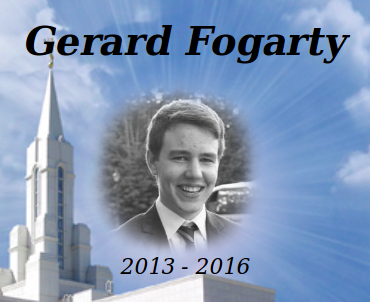
\includegraphics[width=0.46\columnwidth]{obituary} % Example image
\end{center}
\end{homeworkProblem}
\end{document}
\newpage
%----------------------------------------------------------------------------------------
\begin{homeworkProblem}[Conclusion]
\begin{homeworkSection}{The loss of a team member}
We suffered a tragic loss,,, Gerard has become a lost lamp
\end{homeworkSection}
\end{homeworkProblem}
\end{document}